\documentclass[12pt]{article}  % Removed 'runningheads'

\usepackage[utf8]{inputenc}
\usepackage{amsmath,amssymb,hyperref,array,xcolor,multicol,verbatim,mathpazo}
\usepackage[normalem]{ulem}
\usepackage[pdftex]{graphicx}
\graphicspath{{../Figures/}}
\usepackage{fullpage}
\usepackage{natbib}
\usepackage{caption} % Optional, for caption styling

\makeatletter
\renewcommand{\maketitle}{
  \begin{center}
    {\Large \@title \par}
    \vspace{0.3em}  % You can reduce or set to 0em to tighten further
    {\normalsize \@author \par}
    \@thanks  % This ensures footnote text appears
  \end{center}
}
\makeatother
\renewcommand{\thefootnote}{\fnsymbol{footnote}}

\title{Deviation from a Good Will: Land Misallocation under Imperfect Monitoring in China}
\author{Ze Wang\thanks{PhD Candidate, The University of Tokyo}}

\begin{document}
\maketitle



In response to growing concerns over food security, the Chinese central government has enforced a “Red Line” policy mandating that total arable land remain above 1.8 billion mu. Since 2018, this mandate has been reinforced through a stringent assessment system that incorporates cropland area targets into local officials’ performance evaluations. While well-intentioned, this incentive structure is inherently flawed: it monitors surface area metrics rather than actual land use or agricultural output. As a result, local governments—under pressure to fulfill both land protection and economic development goals—frequently convert environmentally fragile or agriculturally unviable land into nominal cropland.

This study explores how such misaligned incentives, coupled with imperfect monitoring, result in land misallocation. In particular, it highlights the phenomenon of “form over function” in land management, where compliance with surface-level targets undermines broader environmental goals. Using spatial land cover data, this study empirically tests whether regions facing stricter land constraints exhibit higher incidences of inefficient cropland expansion after the 2018 policy reform.

In a difference-in-differences framework, I find that land-scarce regions subject to stricter cropland protection targets experienced a disproportionate increase in cropland area after the 2018 policy reform. This result supports the view that central mandates were binding and influential in shaping local land use responses. However, the observed increase in cropland does not necessarily reflect productive agricultural expansion. Instead, I hypothesize that much of this growth in land-constrained regions occurred on marginal or low-productivity land.\footnote{I am currently working on measuring land misallocation and wish to discuss preliminary findings at the conference.} In prefectures where promotion incentives are stronger---such as those with newly appointed or tenure-seeking officials---I expect to observe greater divergence between reported cropland area and actual land use. These patterns would indicate a misallocation of land resources driven by bureaucratic incentives rather than agronomic or environmental considerations.

This study builds on research in land regulation that explores how policy frameworks shape economic outcomes, including housing prices~\citep{hilber2016impact}, economic growth~\citep{besley2000land}, and agricultural productivity~\citep{beg2022digitization, adamopoulos2022misallocation}. While prior work emphasizes misallocation across farmers, this paper shifts the focus to misallocation across land parcels---a spatial inefficiency overlooked in existing analyses. Second, this study engages with the political economy literature on centralized governance, particularly the multi-tasking problem of local officials under imperfect monitoring \citep{holmstrom1991multitask}. Empirical studies have documented how such governance structures shape environmental regulation enforcement \citep{fan2023land, chen2018career, he2020watering}, yet little attention has been paid to land use outcomes. By highlighting the unintended spillovers from cropland protection policies, this paper bridges the gap between land regulation and bureaucratic incentive design in centralized regimes.


\begin{figure}[htbp]
  \centering
  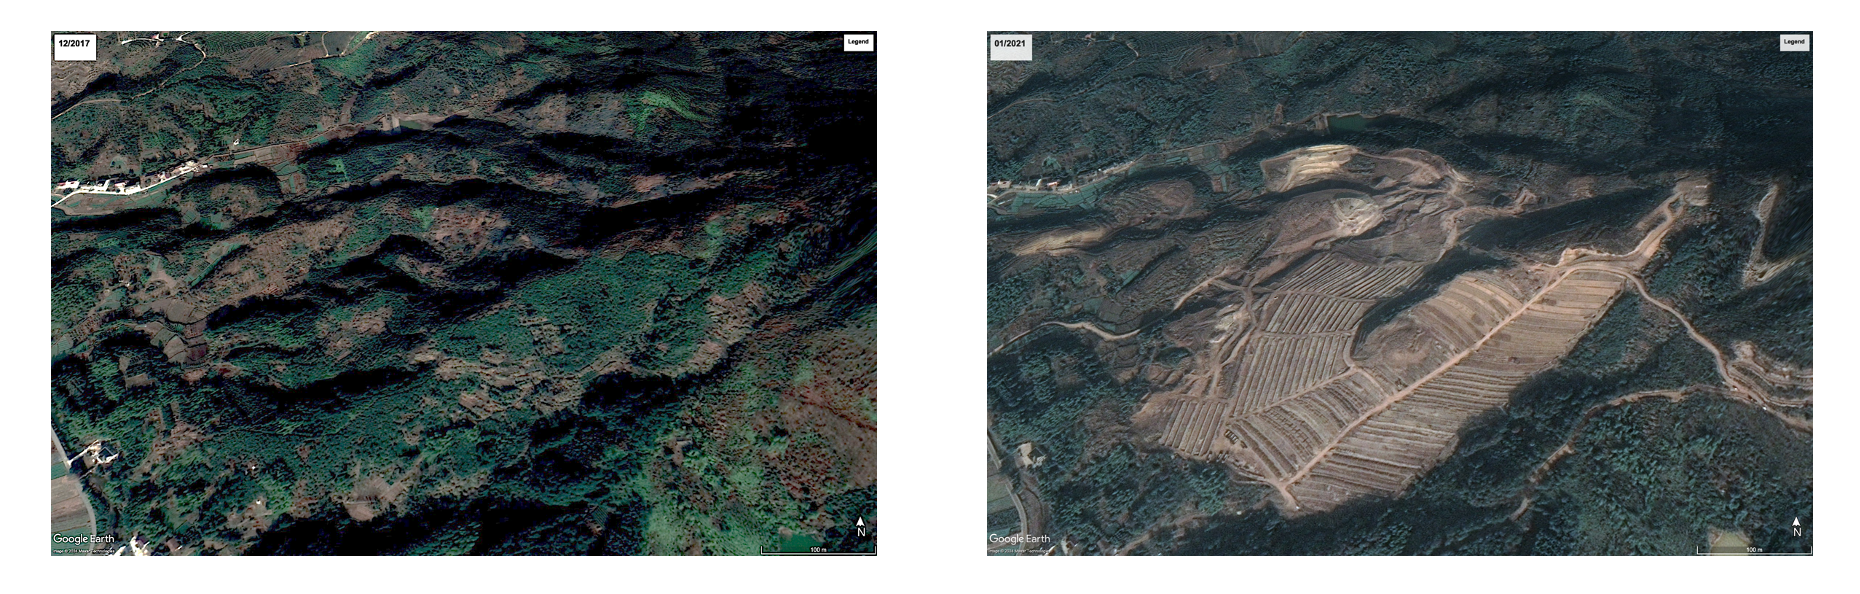
\includegraphics[width=0.8\linewidth]{anecdote_both.png}
  \caption{An example of land conversion from forest to cropland (Google Earth Engine)}
  \label{fig:anecdote}
\end{figure}

{\small
\bibliographystyle{apalike}
\bibliography{literature}
}

\end{document}
